\chapter{Auflagen zur
Akkreditierung\label{/mi-2017/selbstbericht/auflagen/0000-auflagen}}\label{auflagen-zur-akkreditierungpathlabelmi-2017selbstberichtauflagen0000-auflagen}

Die Akkreditierungskommission der ASIIN hat die Studiengänge
Medieninformatik Bachelor und Medieninformatik Master der TH Köln am 30.
Juni 2017 akkreditiert. Hierbei wurden einige Empfehlungen und Auflagen
formuliert. In diesem Dokument finden sich die Erläuterungen zur
fristgerechten Erfüllung der ausgesprochenen Auflagen.

\section{Auflagen für alle
Studiengänge\label{/mi-2017/selbstbericht/auflagen/0000-auflagen}}\label{auflagen-fuxfcr-alle-studienguxe4ngepathlabelmi-2017selbstberichtauflagen0000-auflagen}

\subsection{A1. (AR
2.3)\label{/mi-2017/selbstbericht/auflagen/0000-auflagen}}\label{a1.-ar-2.3pathlabelmi-2017selbstberichtauflagen0000-auflagen}

\begin{siderules}
Die Modulbeschreibungen müssen angemessen über die Voraussetzungen für
die Teilnahme, die Voraussetzungen für die Vergabe von Kreditpunkten und
Notenbildung sowie den Arbeitsaufwand informieren.
\end{siderules}

In den Modulbeschreibungen wurden die entsprechenden Angaben überprüft
und, soweit erforderlich, angepasst. Darüber hinaus wurde innerhalb der
Modulhandbücher jeweils eine kurze Einleitung an den Anfang gestellt.
Diese enthält einen graphischen Studienverlaufsplan, um insgesamt eine
bessere Verständlichkeit und Übersichtlichkeit herzustellen. Darüber
hinaus wurden Hyperlinks innerhalb der Handbücher farblich
hervorgehoben, um eine besser Handhabbarkeit und schnellere Navigation
im jeweiligen Handbuch zu ermöglichen.

Die aktuellen Modulhandbücher sind über folgende URL erreichbar:

\begin{itemize}
\tightlist
\item
  \href{http://www.medieninformatik.th-koeln.de/download/modulbeschreibungen-bachelor-bpo4.pdf}{Modulhandbuch
  Medieninformatik Bachelor}
\item
  \href{http://www.medieninformatik.th-koeln.de/download/modulbeschreibungen-master-mpo4.pdf}{Modulhandbuch
  Medieninformatik Master}
\end{itemize}

\subsection{A2. (AR 2.8)
\label{/mi-2017/selbstbericht/auflagen/0000-auflagen}}\label{a2.-ar-2.8-pathlabelmi-2017selbstberichtauflagen0000-auflagen}

\begin{siderules}
Die in Kraft gesetzten und veröffentlichten Ordnungen inklusive der
angepassten Diploma Supplements für beide Studiengänge sind vorzulegen.
\end{siderules}

Die Prüfungsordnung und der zugehörige Studienverlaufsplan für den
Medieninformatik Bachelor wurden mit der \textbf{Änderungssatzung vom
24.11.2017} in Kraft gesetzt und auf der Website der TH Köln
veröffentlicht:
\href{https://www.th-koeln.de/studium/medieninformatik-bachelor--ordnungen-und-formulare_3963.php}{Medieninformatik
(Bachelor) -- Ordnungen und Formulare}.

Hier findet sich ein Muster für das zugehörige
\href{https://th-koeln.github.io/mi-2017/download/auflagen/THK-DS-MIF-MIB-PO4.pdf}{Diploma
Supplement für den Medieninformatik Bachelor}

Die Prüfungsordnung und der zugehörige Studienverlaufsplan für den
Medieninformatik Master wurden mit der \textbf{Prüfungsordnung vom
13.07.2017} in Kraft gesetzt und auf der Website der TH Köln
veröffentlicht:
\href{https://www.th-koeln.de/studium/medieninformatik-master--ordnungen-und-formulare_3724.php}{Medieninformatik
(Master) -- Ordnungen und Formulare}.

Hier findet sich ein Muster für das zugehörige
\href{https://th-koeln.github.io/mi-2017/download/auflagen/THK-DS-MIF-MIM-PO4.pdf}{Diploma
Supplement für den Medieninformatik Master}.

Bitte beachten Sie, dass das Diploma Supplement auf speziellem Papier
gedruckt wird, auf dem ein Farbkeil (links) vorgedruckt ist, daher ist
dieser in der PDF-Datei nicht enthalten. Die mit ``«\ldots{}»''
gekennzeichneten Felder, werden bei Ausgabe mit den personalisierten
Daten der jeweiligen Absolvent*innen befüllt.

\section{Auflagen für den
Masterstudiengang\label{/mi-2017/selbstbericht/auflagen/0000-auflagen}}\label{auflagen-fuxfcr-den-masterstudiengangpathlabelmi-2017selbstberichtauflagen0000-auflagen}

\subsection{A3. (AR 2.1)
\label{/mi-2017/selbstbericht/auflagen/0000-auflagen}}\label{a3.-ar-2.1-pathlabelmi-2017selbstberichtauflagen0000-auflagen}

\begin{siderules}
Für die fünf Spezialisierungen des Masterstudiengangs ist eine
gleichmäßige detaillierte Beschreibung der Berufsfelder in den
Qualifikationszielen vorzunehmen. Die Module sind als eigenständige
Lehr-/Lerneinheiten darzustellen (unabhängig von der Darstellung der
Schwerpunkte, zu denen sie gehören).
\end{siderules}

Die Beschreibung der Spezialisierungen des Masterstudiengangs wurden im
Modulhandbuch um den Punkt «Berufsbilder» ergänzt. Aufgrund der
fachbedingten Unterschiede der Spezialisierungen, sind diese
Erläuterungen teilweise unterschiedlich aufgebaut, verfolgen aber alle
das Ziel, den Studierenden und Studieninteressierten klar zu machen,
welche beruflichen Perspektiven sich mit der jeweiligen Spezialisierung
eröffnen.

Die Schwerpunktspezifische Pflichtmodule der jeweiligen Spezialisierung
sind jetzt als farblich gekennzeichnete Hyperlinks im Handbuch
hinterlegt und führen direkt zur entsprechenden Modulbeschreibung des
jeweiligen Moduls. Die Modulbeschreibungen selbst, enthalten im
Factsheet zum Modul jetzt den Punkt «Pflichtmodul(e) im Schwerpunkt», um
die entsprechenden Zugehörigkeiten transparent zu machen.

Das überarbeitete Modulhandbucher ist über folgende URL erreichbar:

\begin{itemize}
\tightlist
\item
  \href{http://www.medieninformatik.th-koeln.de/download/modulbeschreibungen-master-mpo4.pdf}{Modulhandbuch
  Medieninformatik Master}
\end{itemize}

\begin{figure}[htbp]
\centering
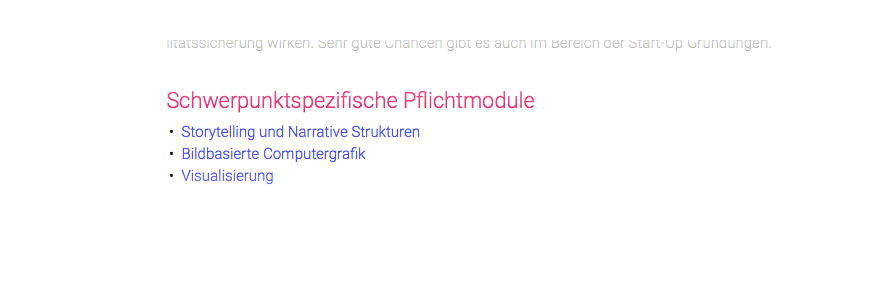
\includegraphics[width=\textwidth]{../anhaenge/bilder/hyperlinks.png}
\caption{Hyperlinks zu den Modulbeschreibungen}
\end{figure}

\begin{figure}[htbp]
\centering
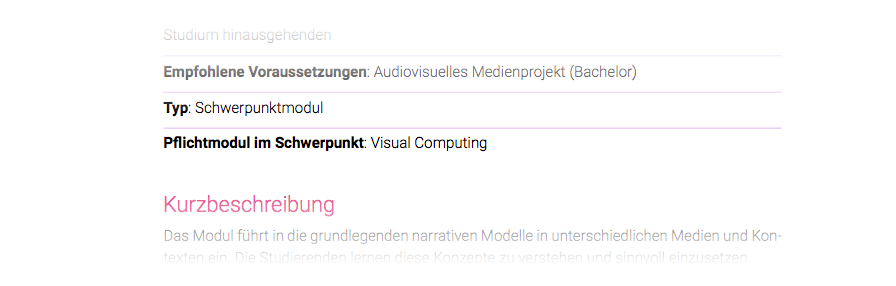
\includegraphics[width=\textwidth]{../anhaenge/bilder/pm-im-schwerpunkt.png}
\caption{Schwerpunktzugehörigkeit des jeweiligen Moduls}
\end{figure}
